\documentclass[12pt]{beamer}\usepackage[]{graphicx}\usepackage[]{color}
%% maxwidth is the original width if it is less than linewidth
%% otherwise use linewidth (to make sure the graphics do not exceed the margin)
\makeatletter
\def\maxwidth{ %
  \ifdim\Gin@nat@width>\linewidth
    \linewidth
  \else
    \Gin@nat@width
  \fi
}
\makeatother

\definecolor{fgcolor}{rgb}{0.345, 0.345, 0.345}
\newcommand{\hlnum}[1]{\textcolor[rgb]{0.686,0.059,0.569}{#1}}%
\newcommand{\hlstr}[1]{\textcolor[rgb]{0.192,0.494,0.8}{#1}}%
\newcommand{\hlcom}[1]{\textcolor[rgb]{0.678,0.584,0.686}{\textit{#1}}}%
\newcommand{\hlopt}[1]{\textcolor[rgb]{0,0,0}{#1}}%
\newcommand{\hlstd}[1]{\textcolor[rgb]{0.345,0.345,0.345}{#1}}%
\newcommand{\hlkwa}[1]{\textcolor[rgb]{0.161,0.373,0.58}{\textbf{#1}}}%
\newcommand{\hlkwb}[1]{\textcolor[rgb]{0.69,0.353,0.396}{#1}}%
\newcommand{\hlkwc}[1]{\textcolor[rgb]{0.333,0.667,0.333}{#1}}%
\newcommand{\hlkwd}[1]{\textcolor[rgb]{0.737,0.353,0.396}{\textbf{#1}}}%

\usepackage{framed}
\makeatletter
\newenvironment{kframe}{%
 \def\at@end@of@kframe{}%
 \ifinner\ifhmode%
  \def\at@end@of@kframe{\end{minipage}}%
  \begin{minipage}{\columnwidth}%
 \fi\fi%
 \def\FrameCommand##1{\hskip\@totalleftmargin \hskip-\fboxsep
 \colorbox{shadecolor}{##1}\hskip-\fboxsep
     % There is no \\@totalrightmargin, so:
     \hskip-\linewidth \hskip-\@totalleftmargin \hskip\columnwidth}%
 \MakeFramed {\advance\hsize-\width
   \@totalleftmargin\z@ \linewidth\hsize
   \@setminipage}}%
 {\par\unskip\endMakeFramed%
 \at@end@of@kframe}
\makeatother

\definecolor{shadecolor}{rgb}{.97, .97, .97}
\definecolor{messagecolor}{rgb}{0, 0, 0}
\definecolor{warningcolor}{rgb}{1, 0, 1}
\definecolor{errorcolor}{rgb}{1, 0, 0}
\newenvironment{knitrout}{}{} % an empty environment to be redefined in TeX

\usepackage{alltt}
\usepackage{graphicx}
\usepackage{tikz}
\setbeameroption{hide notes}
\setbeamertemplate{note page}[plain]
\usepackage{listings}

% get rid of junk
\usetheme{default}
\usefonttheme[onlymath]{serif}
\beamertemplatenavigationsymbolsempty
\hypersetup{pdfpagemode=UseNone} % don't show bookmarks on initial view

% named colors
\definecolor{offwhite}{RGB}{255,250,240}
\definecolor{gray}{RGB}{155,155,155}

\ifx\notescolors\undefined % slides

  \definecolor{foreground}{RGB}{80,80,80}
  \definecolor{background}{RGB}{255,255,255}
  \definecolor{title}{RGB}{255,199,0}
  \definecolor{subtitle}{RGB}{89,132,212}
  \definecolor{hilit}{RGB}{248,117,79}
  \definecolor{vhilit}{RGB}{255,111,207}
  \definecolor{lolit}{RGB}{200,200,200}
  \definecolor{lit}{RGB}{255,199,0}
  \definecolor{mdlit}{RGB}{89,132,212}
  \definecolor{link}{RGB}{248,117,79}

\else % notes
  \definecolor{background}{RGB}{255,255,255}
  \definecolor{foreground}{RGB}{24,24,24}
  \definecolor{title}{RGB}{27,94,134}
  \definecolor{subtitle}{RGB}{22,175,124}
  \definecolor{hilit}{RGB}{122,0,128}
  \definecolor{vhilit}{RGB}{255,0,128}
  \definecolor{lolit}{RGB}{95,95,95}
\fi
\definecolor{nhilit}{RGB}{128,0,128}  % hilit color in notes
\definecolor{nvhilit}{RGB}{255,0,128} % vhilit for notes

\newcommand{\hilit}{\color{hilit}}
\newcommand{\vhilit}{\color{vhilit}}
\newcommand{\nhilit}{\color{nhilit}}
\newcommand{\nvhilit}{\color{nvhilit}}
\newcommand{\lit}{\color{lit}}
\newcommand{\mdlit}{\color{mdlit}}
\newcommand{\lolit}{\color{lolit}}

% use those colors
\setbeamercolor{titlelike}{fg=title}
\setbeamercolor{subtitle}{fg=subtitle}
\setbeamercolor{frametitle}{fg=gray}
\setbeamercolor{structure}{fg=subtitle}
\setbeamercolor{institute}{fg=lolit}
\setbeamercolor{normal text}{fg=foreground,bg=background}
%\setbeamercolor{item}{fg=foreground} % color of bullets
%\setbeamercolor{subitem}{fg=hilit}
%\setbeamercolor{itemize/enumerate subbody}{fg=lolit}
\setbeamertemplate{itemize subitem}{{\textendash}}
\setbeamerfont{itemize/enumerate subbody}{size=\footnotesize}
\setbeamerfont{itemize/enumerate subitem}{size=\footnotesize}

% center title of slides
\setbeamertemplate{blocks}[rounded]
\setbeamertemplate{frametitle}[default][center]
% margins
\setbeamersize{text margin left=25pt,text margin right=25pt}

% page number
\setbeamertemplate{footline}{%
    \raisebox{5pt}{\makebox[\paperwidth]{\hfill\makebox[20pt]{\lolit
          \scriptsize\insertframenumber}}}\hspace*{5pt}}

% add a bit of space at the top of the notes page
\addtobeamertemplate{note page}{\setlength{\parskip}{12pt}}

% default link color
\hypersetup{colorlinks, urlcolor={link}}

\ifx\notescolors\undefined % slides
  % set up listing environment
  \lstset{language=bash,
          basicstyle=\ttfamily\scriptsize,
          frame=single,
          commentstyle=,
          backgroundcolor=\color{darkgray},
          showspaces=false,
          showstringspaces=false
          }
\else % notes
  \lstset{language=bash,
          basicstyle=\ttfamily\scriptsize,
          frame=single,
          commentstyle=,
          backgroundcolor=\color{offwhite},
          showspaces=false,
          showstringspaces=false
          }
\fi

% a few macros
\newcommand{\code}[1]{\texttt{#1}}
\newcommand{\hicode}[1]{{\hilit \texttt{#1}}}
\newcommand{\bb}[1]{\begin{block}{#1}}
\newcommand{\eb}{\end{block}}
\newcommand{\bi}{\begin{itemize}}
%\newcommand{\bbi}{\vspace{24pt} \begin{itemize} \itemsep8pt}
\newcommand{\bbi}{\vspace{4pt} \begin{itemize} \itemsep8pt}
\newcommand{\ei}{\end{itemize}}
\newcommand{\bv}{\begin{verbatim}}
\newcommand{\ev}{\end{verbatim}}
\newcommand{\ig}{\includegraphics}
\newcommand{\subt}[1]{{\footnotesize \color{subtitle} {#1}}}
\newcommand{\ttsm}{\tt \small}
\newcommand{\ttfn}{\tt \footnotesize}
\newcommand{\figh}[2]{\centerline{\includegraphics[height=#2\textheight]{#1}}}
\newcommand{\figw}[2]{\centerline{\includegraphics[width=#2\textwidth]{#1}}}



%------------------------------------------------
% end of header
%------------------------------------------------

\title{Text Data}
\subtitle{STAT 133}
\author{\href{http://www.gastonsanchez.com}{Gaston Sanchez}}
\institute{Department of Statistics, UC{\textendash}Berkeley}
\date{\href{http://www.gastonsanchez.com}{\tt \scriptsize \color{foreground} gastonsanchez.com}
\\[-4pt]
\href{http://github.com/gastonstat/stat133}{\tt \scriptsize \color{foreground} github.com/gastonstat/stat133}
\\[-4pt]
{\scriptsize Course web: \href{http://www.gastonsanchez.com/stat133}{\tt gastonsanchez.com/stat133}}
}
\IfFileExists{upquote.sty}{\usepackage{upquote}}{}
\begin{document}


{
  \setbeamertemplate{footline}{} % no page number here
  \frame{
    \titlepage
  } 
}

%------------------------------------------------

\begin{frame}
\begin{center}
\Huge{\hilit{Datasets}}
\end{center}
\end{frame}

%------------------------------------------------

\begin{frame}
\frametitle{Datasets}

\bb{You'll have some sort of (raw) data to work with}
\eb
\begin{center}
\ig[width=10cm]{images/tabular_nontabular.pdf}
\end{center}

\end{frame}

%------------------------------------------------

\begin{frame}
\frametitle{Data}

\bbi
  \item Much of the data we deal with are given to us as plain text
  \item The data are merely represented by their text form
  \item Sometimes the data are easily interpreted
\ei

\end{frame}

%------------------------------------------------

\begin{frame}[fragile]
\frametitle{Toy Data (tabular layout)}

\begin{center}
 \begin{tabular}{| l | l | l |}
  \hline
name & gender & height \\
  \hline
Leia Skywalker & female & 1.50 \\
  \hline
Luke Skywalker & male & 1.72 \\
  \hline
Han Solo & male & 1.80 \\
  \hline
 \end{tabular}
\end{center}

\bigskip
Typically we get data formed of strings and numeric values

\end{frame}

%------------------------------------------------

\begin{frame}[fragile]
\frametitle{Comma Delimited (\code{csv})}

{\small
\begin{verbatim}
name,gender,height,weight,jedi,species,weapon
Luke Skywalker,male,1.72,77,jedi,human,lightsaber
Leia Skywalker,female,1.50,49,no_jedi,human,blaster
Obi-Wan Kenobi,male,1.82,77,jedi,human,lightsaber
Han Solo,male,1.80,80,no_jedi,human,blaster
R2-D2,male,0.96,32,no_jedi,droid,unarmed
C-3PO,male,1.67,75,no_jedi,droid,unarmed
Yoda,male,0.66,17,jedi,yoda,lightsaber
Chewbacca,male,2.28,112,no_jedi,wookiee,bowcaster
\end{verbatim}
}

\end{frame}

%------------------------------------------------

\begin{frame}
\frametitle{However ...}

\bbi
  \item There are many examples of more complex situations
  \item It is not uncommon to deal with data that are not as easily interpreted
  \item And thus the text must be processed to create values of interest
\ei

\end{frame}

%------------------------------------------------

\begin{frame}
\frametitle{For instance ...}

\bi
  \item e.g. when numeric values are embedded into text
  \item e.g. numeric values not in a regular or simple format
  \item e.g. numbers in an HTML table
  \item e.g. data in non-delimited-field formats 
\ei

\end{frame}

%------------------------------------------------

\begin{frame}
\begin{center}
\Huge{\hilit{Text Everywhere}}
\end{center}
\end{frame}

%------------------------------------------------

\begin{frame}[fragile]
\frametitle{Text in plots}

\begin{knitrout}\scriptsize
\definecolor{shadecolor}{rgb}{0.969, 0.969, 0.969}\color{fgcolor}

{\centering 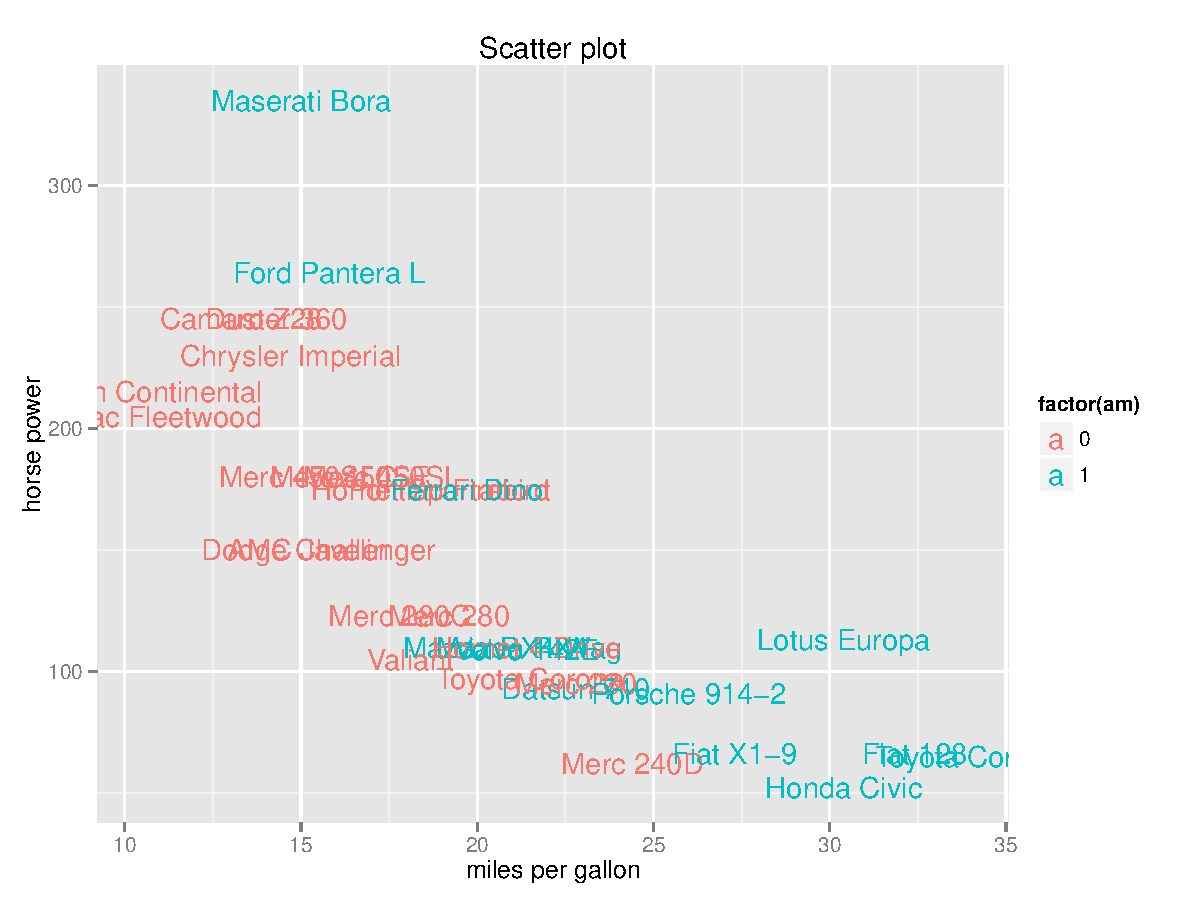
\includegraphics[width=.9\linewidth,height=.7\linewidth]{figure/your_xyplot3-1} 

}



\end{knitrout}

\end{frame}

%------------------------------------------------

\begin{frame}[fragile]
\frametitle{Text in scripts}

\begin{knitrout}\scriptsize
\definecolor{shadecolor}{rgb}{0.969, 0.969, 0.969}\color{fgcolor}\begin{kframe}
\begin{alltt}
\hlcom{# =====================================================}
\hlcom{# Stat133: Lab 2}
\hlcom{# Description: Basics of data frames}
\hlcom{# Data: Star Wars characters}
\hlcom{# =====================================================}

\hlcom{# load "readr}
\hlkwd{library}\hlstd{(}\hlstr{"readr"}\hlstd{)}

\hlcom{# read data using read_csv()}
\hlstd{sw} \hlkwb{<-} \hlkwd{read_csv}\hlstd{(}\hlstr{"~/stat133/datasets/starwarstoy.csv"}\hlstd{)}

\hlcom{# use str() to get information about the data frame structure}
\hlkwd{str}\hlstd{(sw)}

\hlcom{# use summary() to get some descriptive statistics}
\hlkwd{summary}\hlstd{(sw)}

\hlcom{# convert column 'gender' as a factor}
\hlstd{sw}\hlopt{$}\hlstd{gender} \hlkwb{<-} \hlkwd{factor}\hlstd{(sw}\hlopt{$}\hlstd{gender)}
\end{alltt}
\end{kframe}
\end{knitrout}

\end{frame}

%------------------------------------------------

\begin{frame}[fragile]
\frametitle{Text: names of files and directories}
\begin{center}
\ig[width=10cm]{images/dirfiles.png}
\end{center}
\end{frame}

%------------------------------------------------

\begin{frame}[fragile]
\frametitle{Wikipedia Table}

\begin{center}
\ig[width=6.5cm]{images/wikipedia_table.png}

\scalebox{.5}{\url{https://en.wikipedia.org/wiki/World_record_progression_1500_metres_freestyle
}}
\end{center}

\end{frame}

%------------------------------------------------

\begin{frame}[fragile]
\frametitle{Wikipedia Table}
\begin{center}
\ig[width=11cm]{images/wiki_swimming.png}
\end{center}
\end{frame}

%------------------------------------------------

\begin{frame}
\begin{center}
\Huge{\mdlit{Example: XML Data}}
\end{center}
\end{frame}

%------------------------------------------------

\begin{frame}[fragile]
\frametitle{Toy Data (XML format)}

\begin{knitrout}\footnotesize
\definecolor{shadecolor}{rgb}{0.969, 0.969, 0.969}\color{fgcolor}\begin{kframe}
\begin{alltt}
<subject>
  <name>
    <first>Luke</first>
    <last>Skywalker</last>
  </name>
  <gender>male</gender>
  <height>1.72</height>
</subject>
<subject>
  <name>
    <first>Leia</first>
    <last>Skywalker</last>
  </name>
  <gender>female</gender>
  <height>1.50</height>
</subject>
\end{alltt}
\end{kframe}
\end{knitrout}

\end{frame}

%------------------------------------------------

\begin{frame}[fragile]
\frametitle{Toy Data (XML format)}

Looking at one {\hilit \code{<subject>}} node:
\begin{knitrout}\footnotesize
\definecolor{shadecolor}{rgb}{0.969, 0.969, 0.969}\color{fgcolor}\begin{kframe}
\begin{alltt}
<subject>
  <name>
    <first>Luke</first>
    <last>Skywalker</last>
  </name>
  <gender>male</gender>
  <height>1.72</height>
</subject>
\end{alltt}
\end{kframe}
\end{knitrout}

\end{frame}

%------------------------------------------------

\begin{frame}
\frametitle{XML hierarchical structure}
\begin{center}
\ig[width=10cm]{images/xml_nodes.pdf}
\end{center}
\end{frame}

%------------------------------------------------

\begin{frame}
\frametitle{Extracting Data}

\bbi
  \item Sometimes we must extract the elements of interest from the text content
  \item The extraction is done by identifying the patterns where the values occur
\ei

\end{frame}

%------------------------------------------------

\begin{frame}
\frametitle{Extracting Data}

\bi
  \item A different example occurs when text itself makes up the data
  \item Speech
  \item Lyrics
  \item Email messages
  \item Abstract
  \item \textit{etc}
\ei

\end{frame}

%------------------------------------------------

\begin{frame}[fragile]
\frametitle{Example: Speech}

{\small Text of President Barack Obama's State of the Union address, as provided by the White House:

\begin{quotation}
Mr. Speaker, Mr. Vice President, members of Congress, distinguished guests and fellow Americans:

Last month, I went to Andrews Air Force Base and welcomed home some of our last troops to serve in Iraq. Together, we offered a final, proud salute to the colors under which more than a million of our fellow citizens fought-- and several thousand gave their lives.
\end{quotation}
}

\end{frame}

%------------------------------------------------

\begin{frame}
\frametitle{Example: Abstract}
\begin{center}
\ig[width=8cm]{images/pubmed_article.png}
\end{center}
\end{frame}

%------------------------------------------------

\begin{frame}
\begin{center}
\Huge{\mdlit{Example: Web Log}}
\end{center}
\end{frame}

%------------------------------------------------

\begin{frame}[fragile]
\frametitle{Web log example}

\begin{verbatim}
123.123.123.123 - - [26/Apr/2000:00:23:48 -0400] 
"GET /pics/wpaper.gif HTTP/1.0" 200 6248 
"http://www.jafsoft.com/asctortf/" 
"Mozilla/4.05 (Macintosh; I; PPC)"


123.123.123.123 - - [26/Apr/2000:00:23:47 -0400] 
"GET /asctortf/ HTTP/1.0" 200 8130 
"http://search.netscape.com/Computers/Data_Formats" 
"Mozilla/4.05 (Macintosh; I; PPC)"
\end{verbatim}

\end{frame}

%------------------------------------------------

\begin{frame}
\frametitle{Web log data}

\bi
  \item The information in the log has a lot of structure
  \item e.g. the date always appears in square brackets
  \item However, the information is not consistently separated by the same characters
  \item Nor is it placed consistently in the same columns in the file
\ei

\end{frame}

%------------------------------------------------

\begin{frame}[fragile]
\frametitle{Web log example}

Web log content structure:
\bigskip

{\small
\begin{verbatim}
ppp931.on.bellglobal.com
- -
[26/Apr/2000:00:16:12 -0400]
"GET /download/windows/asctab31.zip HTTP/1.0"
200
1540096
"http://www.htmlgoodies.com/downloads/freeware/15.html"
"Mozilla/4.7 [en]C-SYMPA  (Win95; U)"
\end{verbatim}
}

\end{frame}

%------------------------------------------------

\begin{frame}
\frametitle{Web log data}

\bi
  \item IP address: {\hilit \code{ppp931.on.bellglobal.com}}
  \item Username etc: {\hilit \code{"- -"}}
  \item Timestamp: {\hilit \code{"[26/Apr/2000:00:16:12 -0400]"}}
  \item Access request: \\ 
  {\hilit \code{"GET /download/windows/asctab31.zip HTTP/1.0"}}
  \item Result status code: {\hilit \code{"200"}}
  \item Bytes transferred: {\hilit \code{"1540096"}}
  \item Referrer URL: \\ {\hilit \footnotesize \code{"http://www.htmlgoodies.com/downloads/freeware/15.html"}}
  \item User Agent: {\hilit \code{"Mozilla/4.7 [en]C-SYMPA (Win95; U)"}}
\ei

\end{frame}

%------------------------------------------------

\begin{frame}
\frametitle{Spam Filtering}

\bb{Anatomy of an email message}
\bi
  \item Three parts:
  \bi
    \item header
    \item body
    \item attachments (optional)
  \ei
  \item Like regular mail, the header is the envelope and the body is the letter
  \item Plain text
\ei
\eb

\end{frame}

%------------------------------------------------

\begin{frame}
\frametitle{Spam Filtering}

\bb{Email header}
\bi
  \item date, sender, and subject
  \item message id
  \item who are the carbon-copy recipients
  \item return path
\ei
\eb

\end{frame}

%------------------------------------------------

\begin{frame}[fragile]
\frametitle{Example Email Header}

\begin{verbatim}
Date: Mon, 29 Jun 2015 22:16:19 -0800 (PST)
From: doe@email.edu
X-X-Sender: smith@email.net
To: Txxxx Uxxx <txxxx@uclink.berkeley.edu>
Subject: Re: prof: did you receive my hw?
In-Reply-To: <web-569552@calmail-st.berkeley.edu>
MIME-Version: 1.0
Content-Type: TEXT/PLAIN; charset=US-ASCII
Status: 0
X-Status: 
X-Keywords:
X-UID: 9079
\end{verbatim}

\end{frame}

%------------------------------------------------

\begin{frame}
\begin{center}
\Huge{\hilit{Example: Movie Scripts}}
\end{center}
\end{frame}

%------------------------------------------------

\begin{frame}
\frametitle{}
\begin{center}
\ig[width=11cm]{images/starwars.jpg}
\end{center}
\end{frame}

%------------------------------------------------

\begin{frame}
\frametitle{}
\begin{center}
\ig[width=11cm]{images/episodes.pdf}
\end{center}
\end{frame}

%------------------------------------------------

\begin{frame}[fragile]
\frametitle{}

\begin{verbatim}
                    STAR WARS

                    Episode V
                                   
             THE EMPIRE STRIKES BACK

               Script adaptation by
        Lawrence Kasdan and Leigh Brackett
                 from a story by
                   George Lucas

                  LUCASFILM LTD.
\end{verbatim}

\end{frame}

%------------------------------------------------

\begin{frame}[fragile]
\frametitle{Reading Text}



\begin{knitrout}\footnotesize
\definecolor{shadecolor}{rgb}{0.969, 0.969, 0.969}\color{fgcolor}\begin{kframe}
\begin{alltt}
\hlcom{# read data as string vector}
\hlstd{sw} \hlkwb{<-} \hlkwd{readLines}\hlstd{(}\hlstr{"StarWars_EpisodeV_script.txt"}\hlstd{)}

\hlstd{sw[}\hlnum{1}\hlopt{:}\hlnum{13}\hlstd{]}
\end{alltt}
\end{kframe}
\end{knitrout}

\begin{knitrout}\scriptsize
\definecolor{shadecolor}{rgb}{0.969, 0.969, 0.969}\color{fgcolor}\begin{kframe}
\begin{verbatim}
##  [1] ""                                                    
##  [2] "                              STAR WARS"             
##  [3] ""                                                    
##  [4] "                              Episode V"             
##  [5] "                                   "                 
##  [6] "                       THE EMPIRE STRIKES BACK"      
##  [7] ""                                                    
##  [8] "                         Script adaptation by"       
##  [9] "                  Lawrence Kasdan and Leigh Brackett"
## [10] "                           from a story by"          
## [11] "                             George Lucas"           
## [12] ""                                                    
## [13] "                            LUCASFILM LTD."
\end{verbatim}
\end{kframe}
\end{knitrout}

\end{frame}

%------------------------------------------------

\begin{frame}[fragile]
\frametitle{Star Wars Episode V script}

{\scriptsize
\begin{verbatim}
A long time ago, in a galaxy far, far, away...


   It is a dark time for the Rebellion. Although the Death Star has
been destroyed, Imperial troops have driven the Rebel forces from
their hidden base and pursued them across the galaxy.
   Evading the dreaded Imperial Starfleet, a group of freedom fighters
led by Luke Skywalker has established a new secret base on the remote
ice world of Hoth.
   The evil lord Darth Vader, obsessed with finding young Skywalker,
has dispatched thousands of remote probes into the far reaches of
space...
\end{verbatim}
}

\end{frame}

%------------------------------------------------

\begin{frame}[fragile]
\frametitle{Star Wars Episode V script}

{\scriptsize
\begin{verbatim}
LUKE: (into comlink) Echo Three to Echo Seven. Han, old buddy, do you
read me?


          After a little static a familiar voice is heard.


HAN: (over comlink) Loud and clear, kid. What's up?


LUKE: (into comlink) Well, I finished my circle. I don't pick up any 
life readings.


HAN: (over comlink) There isn't enough life on this ice cube to fill a 
space cruiser. The sensors are placed. I'm going back.
\end{verbatim}
}

\end{frame}

%------------------------------------------------

\begin{frame}[fragile]
\frametitle{Reading Text}

\begin{knitrout}\tiny
\definecolor{shadecolor}{rgb}{0.969, 0.969, 0.969}\color{fgcolor}\begin{kframe}
\begin{alltt}
\hlstd{sw[}\hlnum{64}\hlopt{:}\hlnum{74}\hlstd{]}
\end{alltt}
\begin{verbatim}
##  [1] "LUKE: (into comlink) Echo Three to Echo Seven. Han, old buddy, do you" 
##  [2] "read me?"                                                              
##  [3] "           After a little static a familiar voice is heard."           
##  [4] ""                                                                      
##  [5] "HAN: (over comlink) Loud and clear, kid. What's up?"                   
##  [6] ""                                                                      
##  [7] "LUKE: (into comlink) Well, I finished my circle. I don't pick up any"  
##  [8] "life readings."                                                        
##  [9] ""                                                                      
## [10] "HAN: (over comlink) There isn't enough life on this ice cube to fill a"
## [11] "space cruiser. The sensors are placed. I'm going back."
\end{verbatim}
\end{kframe}
\end{knitrout}

\end{frame}

%------------------------------------------------

\begin{frame}[fragile]
\frametitle{Matching Text}

\begin{knitrout}\scriptsize
\definecolor{shadecolor}{rgb}{0.969, 0.969, 0.969}\color{fgcolor}\begin{kframe}
\begin{alltt}
\hlkwd{grep}\hlstd{(}\hlstr{'LUKE'}\hlstd{, sw[}\hlnum{64}\hlopt{:}\hlnum{74}\hlstd{])}
\end{alltt}
\begin{verbatim}
## [1] 1 7
\end{verbatim}
\begin{alltt}
\hlkwd{grep}\hlstd{(}\hlstr{'LUKE'}\hlstd{, sw[}\hlnum{64}\hlopt{:}\hlnum{74}\hlstd{],} \hlkwc{value} \hlstd{=} \hlnum{TRUE}\hlstd{)}
\end{alltt}
\begin{verbatim}
## [1] "LUKE: (into comlink) Echo Three to Echo Seven. Han, old buddy, do you"
## [2] "LUKE: (into comlink) Well, I finished my circle. I don't pick up any"
\end{verbatim}
\end{kframe}
\end{knitrout}

\end{frame}

%------------------------------------------------

\begin{frame}[fragile]
\frametitle{Matching Text}

\begin{knitrout}\tiny
\definecolor{shadecolor}{rgb}{0.969, 0.969, 0.969}\color{fgcolor}\begin{kframe}
\begin{alltt}
\hlstd{force_lines} \hlkwb{<-} \hlkwd{grep}\hlstd{(}\hlstr{'force'}\hlstd{, sw)}

\hlkwd{length}\hlstd{(force_lines)}
\end{alltt}
\begin{verbatim}
## [1] 6
\end{verbatim}
\begin{alltt}
\hlstd{sw[force_lines]}
\end{alltt}
\begin{verbatim}
## [1] "been destroyed, Imperial troops have driven the Rebel forces from"    
## [2] "        seconds, other Imperial reinforcements join the scuffle,"     
## [3] "        Luke's feet forces the youth to jump back to protect himself."
## [4] "           Suddenly, Vader attacks so forcefully that Luke loses his" 
## [5] "        exchange and Luke forces Vader back. Another exchange and"    
## [6] "        finally forces him back, away from the edge. The wind soon"
\end{verbatim}
\end{kframe}
\end{knitrout}

\end{frame}

%------------------------------------------------

\begin{frame}[fragile]
\frametitle{Matching Text}

\begin{knitrout}\tiny
\definecolor{shadecolor}{rgb}{0.969, 0.969, 0.969}\color{fgcolor}\begin{kframe}
\begin{alltt}
\hlstd{(force_lines} \hlkwb{<-} \hlkwd{grep}\hlstd{(}\hlstr{'Force'}\hlstd{, sw))}
\end{alltt}
\begin{verbatim}
##  [1] 2550 2562 2877 2878 2890 2912 3126 3180 3184 3339 3340 3634 3637 3656
## [15] 4218 4421 4984
\end{verbatim}
\begin{alltt}
\hlstd{sw[force_lines]}
\end{alltt}
\begin{verbatim}
##  [1] "EMPEROR: There is a great disturbance in the Force."                   
##  [2] "EMPEROR: The Force is strong with him. The son of Skywalker must not"  
##  [3] "YODA: Run! Yes. A Jedi's strength flows from the Force. But beware of" 
##  [4] "the dark side. Anger...fear...aggression. The dark side of the Force"  
##  [5] "the Force for knowledge and defense, never for attack."                
##  [6] "YODA: That place...is strong with the dark side of the Force. A domain"
##  [7] "YODA: Use the Force. Yes..."                                           
##  [8] "YODA: And well you should not. For my ally in the Force. And a"        
##  [9] "feel the Force around you. (gesturing) Here, between you...me...the"   
## [10] "YODA: Concentrate...feel the Force flow. Yes. Good. Calm, yes. Through"
## [11] "the Force, things you will see. Other places. The future...the past."  
## [12] "LUKE: But I can help them! I feel the Force!"                          
## [13] "you will be tempted by the dark side of the Force."                    
## [14] "Knight with the Force as his ally will conquer Vader and his Emperor." 
## [15] "VADER: The Force is with you, young Skywalker. But you are not a Jedi" 
## [16] "        hurtling at him. Using the Force, Luke manages to deflect it"  
## [17] "LUKE: (into comlink) Take care, you two. May the Force be with you."
\end{verbatim}
\end{kframe}
\end{knitrout}

\end{frame}

%------------------------------------------------

\begin{frame}[fragile]
\frametitle{Matching Text}

\begin{knitrout}\tiny
\definecolor{shadecolor}{rgb}{0.969, 0.969, 0.969}\color{fgcolor}\begin{kframe}
\begin{alltt}
\hlstd{(dark_lines} \hlkwb{<-} \hlkwd{grep}\hlstd{(}\hlstr{'dark side'}\hlstd{, sw))}
\end{alltt}
\begin{verbatim}
## [1] 2878 2883 2912 3637 3677 4573
\end{verbatim}
\begin{alltt}
\hlstd{sw[dark_lines]}
\end{alltt}
\begin{verbatim}
## [1] "the dark side. Anger...fear...aggression. The dark side of the Force"  
## [2] "LUKE: Vader. Is the dark side stronger?"                               
## [3] "YODA: That place...is strong with the dark side of the Force. A domain"
## [4] "you will be tempted by the dark side of the Force."                    
## [5] "BEN: Luke, don't give in to hate -- that leads to the dark side."      
## [6] "VADER: If you only knew the power of the dark side. Obi-Wan never told"
\end{verbatim}
\end{kframe}
\end{knitrout}

\end{frame}

%------------------------------------------------

\begin{frame}
\frametitle{Example: Movie Script}

What things would you analyze from a movie script?
\pause
\bi
  \item How many characters?
  \item Most common words?
  \item Number of dialogues per character?
  \item Average number of words per dialogue?
  \item What's the longest word?
\ei

\end{frame}

%------------------------------------------------

\begin{frame}[fragile]
\frametitle{Extracting Text}

\begin{knitrout}\scriptsize
\definecolor{shadecolor}{rgb}{0.969, 0.969, 0.969}\color{fgcolor}\begin{kframe}
\begin{alltt}
\hlkwd{library}\hlstd{(stringr)}

\hlcom{# extract first word}
\hlkwd{str_extract}\hlstd{(sw[}\hlnum{64}\hlopt{:}\hlnum{74}\hlstd{],} \hlstr{"\textbackslash{}\textbackslash{}w+"}\hlstd{)}
\end{alltt}
\begin{verbatim}
##  [1] "LUKE"  "read"  "After" NA      "HAN"   NA      "LUKE"  "life"  NA     
## [10] "HAN"   "space"
\end{verbatim}
\end{kframe}
\end{knitrout}

\end{frame}

%------------------------------------------------

\begin{frame}[fragile]
\frametitle{Replacing Text}

\begin{knitrout}\tiny
\definecolor{shadecolor}{rgb}{0.969, 0.969, 0.969}\color{fgcolor}\begin{kframe}
\begin{alltt}
\hlcom{# replace 'LUKE' by 'Luke'}
\hlkwd{str_replace}\hlstd{(sw[}\hlnum{64}\hlopt{:}\hlnum{74}\hlstd{],} \hlstr{"LUKE"}\hlstd{,} \hlstr{"Luke"}\hlstd{)}
\end{alltt}
\begin{verbatim}
##  [1] "Luke: (into comlink) Echo Three to Echo Seven. Han, old buddy, do you" 
##  [2] "read me?"                                                              
##  [3] "           After a little static a familiar voice is heard."           
##  [4] ""                                                                      
##  [5] "HAN: (over comlink) Loud and clear, kid. What's up?"                   
##  [6] ""                                                                      
##  [7] "Luke: (into comlink) Well, I finished my circle. I don't pick up any"  
##  [8] "life readings."                                                        
##  [9] ""                                                                      
## [10] "HAN: (over comlink) There isn't enough life on this ice cube to fill a"
## [11] "space cruiser. The sensors are placed. I'm going back."
\end{verbatim}
\end{kframe}
\end{knitrout}

\end{frame}

%------------------------------------------------

\begin{frame}[fragile]
\frametitle{Splitting Text}

\begin{knitrout}\tiny
\definecolor{shadecolor}{rgb}{0.969, 0.969, 0.969}\color{fgcolor}\begin{kframe}
\begin{alltt}
\hlcom{# splitting a string into single characters}
\hlkwd{strsplit}\hlstd{(sw[}\hlnum{64}\hlstd{],} \hlstr{""}\hlstd{)}
\end{alltt}
\begin{verbatim}
## [[1]]
##  [1] "L" "U" "K" "E" ":" " " "(" "i" "n" "t" "o" " " "c" "o" "m" "l" "i" "n"
## [19] "k" ")" " " "E" "c" "h" "o" " " "T" "h" "r" "e" "e" " " "t" "o" " " "E"
## [37] "c" "h" "o" " " "S" "e" "v" "e" "n" "." " " "H" "a" "n" "," " " "o" "l"
## [55] "d" " " "b" "u" "d" "d" "y" "," " " "d" "o" " " "y" "o" "u"
\end{verbatim}
\end{kframe}
\end{knitrout}

\end{frame}

%------------------------------------------------

\begin{frame}
\frametitle{Parsing Scripts}

\bb{Dialogues}
\bi
  \item Extracting the dialogues
  \item Identifying Star Wars characters (Luke, Han)
  \item Ignoring descriptions or non-dialogue remarks
  \bi
    \item e.g. \code{After a little static a familiar voice is heard}
  \ei
  \item Ignoring annotations: 
  \bi
    \item e.g. \code{(over comlink)}
    \item e.g. \code{(into comlink)}
  \ei
\ei
\eb

\end{frame}


%------------------------------------------------

\begin{frame}[fragile]
\frametitle{Star Wars Episode V script}

{\scriptsize
\begin{verbatim}
HAN: Chewie!

           The Wookiee grumbles a reply.

HAN: All right, don't lose your temper. I'll come right back and give 
you a hand.

           Chewbacca puts his mask back on and returns to his welding
        as Han leaves.
\end{verbatim}
}

\end{frame}

%------------------------------------------------

\begin{frame}[fragile]
\frametitle{Star Wars Episode V script}

{\scriptsize
\begin{verbatim}
BEN: If you choose to face Vader, you will do it alone. I cannot
interfere.

LUKE: I understand. (he moves to his X-wing) Artoo, fire up the
converters.

           Artoo whistles a happy reply.

BEN: Luke, don't give in to hate -- that leads to the dark side.

           Luke nods and climbs into his ship.

YODA: Strong is Vader. Mind what you have learned. Save you it can.

LUKE: I will. And I'll return. I promise.
\end{verbatim}
}

\end{frame}

%------------------------------------------------

\begin{frame}
\frametitle{Text Analysis}

\bb{Dialogues}
\bi
  \item Identifying words
  \item Counting frequencies of words
  \item Common words: prepositions, articles, conjunctions
  \item Exclamation symbols, numbers, 
\ei
\eb

\end{frame}

%------------------------------------------------

\begin{frame}
\frametitle{}
\begin{center}
\ig[width=11cm]{images/top_characters.pdf}
\end{center}
\end{frame}

%------------------------------------------------

\begin{frame}
\frametitle{Top Characters}
\begin{center}
\ig[width=10cm]{images/Top_20_characters.png}
\end{center}
\end{frame}

%------------------------------------------------

\begin{frame}
\frametitle{Excluded Characters}
\begin{center}
\ig[width=8cm]{images/chewie_r2d2.pdf}
\end{center}
\end{frame}

%------------------------------------------------

\end{document}
